\label{sec:redundant_adders}
The source of the errors of the noisy addition is the error rate of the AND, OR and NOT gates; for example, with probability $1-(1-\beta)^2$ the carry bit $c=0$ even when $a=1$ and $b=1$. In order to reduce this error probability of the AND and OR gates, we propose to introduce scalable {\em redundant computation} (similar to the idea of redundancy in messages in order to compensate for channel noise in communication, see, e.g.\ \cite{Sha1948k}). One such idea is to {\em duplicate} the original function and combine the two parallel computations with an OR such that a value of $1$ is computed if at least one of the original units computes a $1$. More formally, we define
\begin{align}
    a \land_2 b & = (a \land b) \lor (a \land b)   \\
    a \lor_2 b  & = (a \lor b) \lor (a \lor b) \,.
\end{align}
This type of redundancy will achieve the desired effect of minimizing the error of not computing $1$. Similarly, we can combine the original units with and AND gate which minimized the error of not computing $0$.

Using this design pattern, we can now increase the redundancy in an exponential fashion by virtue of
\begin{align}
    a \land_{2k} b & = (a \land_k b) \lor (a \land_k b)   \\
    a \lor_{2k} b  & = (a \lor_k b) \lor (a \lor_k b) \,.
\end{align}
Note that this design still uses the original noise OR gate to compute the combination of all outputs. In Figure \ref{fig:noise_prob_dist_redudancy} we have shown the new probability distribution over the four possible values of $(s,c)$ when replacing all the AND and OR gates in Figure \ref{fig:half-and-full-adder} with $16$--redundant AND and OR gates. All the way to $\beta \approx 10\%$, the error remains relatively small compared to the noise-free half-adder!


\begin{figure}
    \begin{minipage}[c]{.45\linewidth}
        \centering
        \begin{tikzpicture}
            % Circuit style
            \ctikzset{
                logic ports=ieee,
                logic ports/scale=0.8,
                % logic ports/fill=lightgray
            }

            % Logic ports
            \node[and port] (ANDa) at (0,0){};
            \node[and port] (ANDb) at (0,-3){};
            \node[or port] (OR) at (2.5,-1.5){};

            % Input and output ports
            \node (a) at (-2,-1) [left] {$a$};
            \node (b) at (-2,-2) [left] {$b$};
            \node (c) at (1,-3) [above] {$c$};
            \node (d) at (1,0) [above] {$d$};
            \node (s) at (3.5,-1.5) [right] {$o$};
            \node (af) [right = 0.5 of a, coordinate] [left] {};
            \node (bf) [right = 1 of b, coordinate] [left] {};

            % % Connection
            \draw (ANDa.out) -| (OR.in 1);
            \draw (ANDb.out) -| (OR.in 2);

            \draw (OR.out) -* (s);
            \draw (ANDa.in 1) -| (af) |- (ANDb.in 2);
            \draw (ANDa.in 2) -| (bf) |- (ANDb.in 1);
            \draw (a) -- (af);
            \draw (b) -- (bf);
        \end{tikzpicture}
    \end{minipage} \hfill
    \begin{minipage}[c]{.45\linewidth}
        \centering
        \begin{tikzpicture}
            % Circuit style
            \ctikzset{
                logic ports=ieee,
                logic ports/scale=0.8,
                % logic ports/fill=lightgray
            }

            % Logic ports
            \node[or port] (ORa) at (0,0){};
            \node[or port] (ORb) at (0,-3){};
            \node[or port] (OR) at (2.5,-1.5){};

            % Input and output ports
            \node (a) at (-2,-1) [left] {$a$};
            \node (b) at (-2,-2) [left] {$b$};
            \node (c) at (1,-3) [above] {$c$};
            \node (d) at (1,0) [above] {$d$};
            \node (s) at (3.5,-1.5) [right] {$o$};
            \node (af) [right = 0.5 of a, coordinate] [left] {};
            \node (bf) [right = 1 of b, coordinate] [left] {};

            % % Connection
            \draw (ORa.out) -| (OR.in 1);
            \draw (ORb.out) -| (OR.in 2);

            \draw (OR.out) -* (s);
            \draw (ORa.in 1) -| (af) |- (ORb.in 2);
            \draw (ORa.in 2) -| (bf) |- (ORb.in 1);
            \draw (a) -- (af);
            \draw (b) -- (bf);
        \end{tikzpicture}
    \end{minipage}
    \caption{{\bf Left:} Logic circuit design of a $2$--redundant AND gate that computes the function $a \land_2 b := (a \land b) \lor (a \land b)$ which has the exact same truth table than $a \land b$. However, this design has the property that for noisy computations, the probability of erroneously computing $1 \land 1$ as $0$ is reduced when summing out all the four values of $(c,d)$. {\bf Right:} Logic circuit design of a $2$--redundant OR gate that computes the function $a \lor_2 b := (a \lor b) \lor (a \lor b)$ which has the exact same truth table than $a \lor b$.}
\end{figure}

\begin{figure}
    \begin{center}
        \begin{tabular}{cc}
            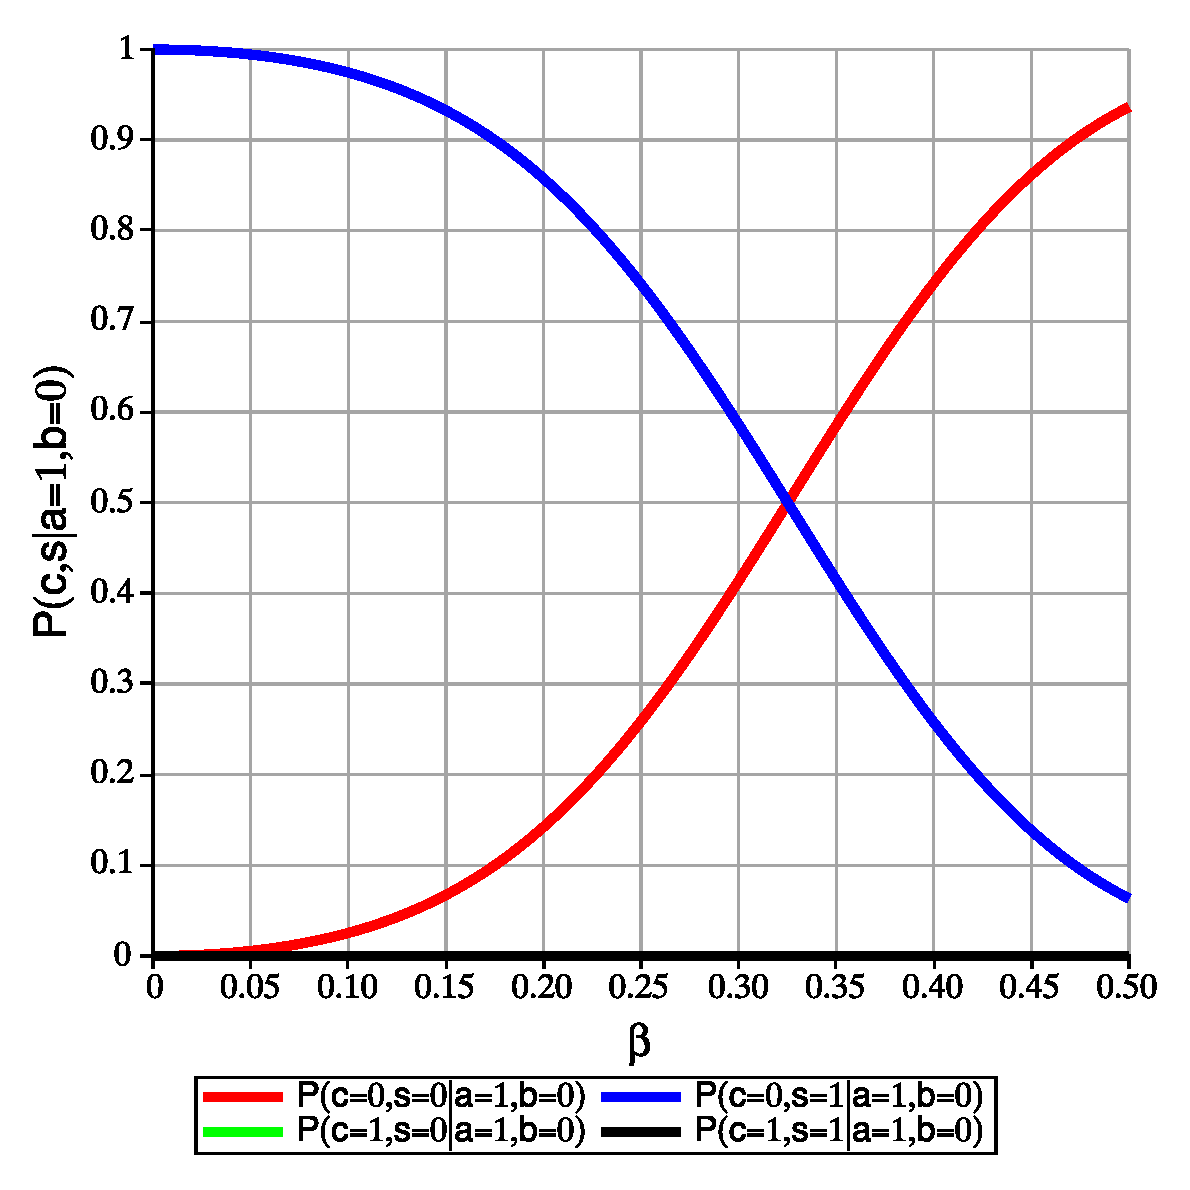
\includegraphics[width=.4\textwidth]{media/noisy_half_adder_16_redundancy_value_dist_10.eps} &
            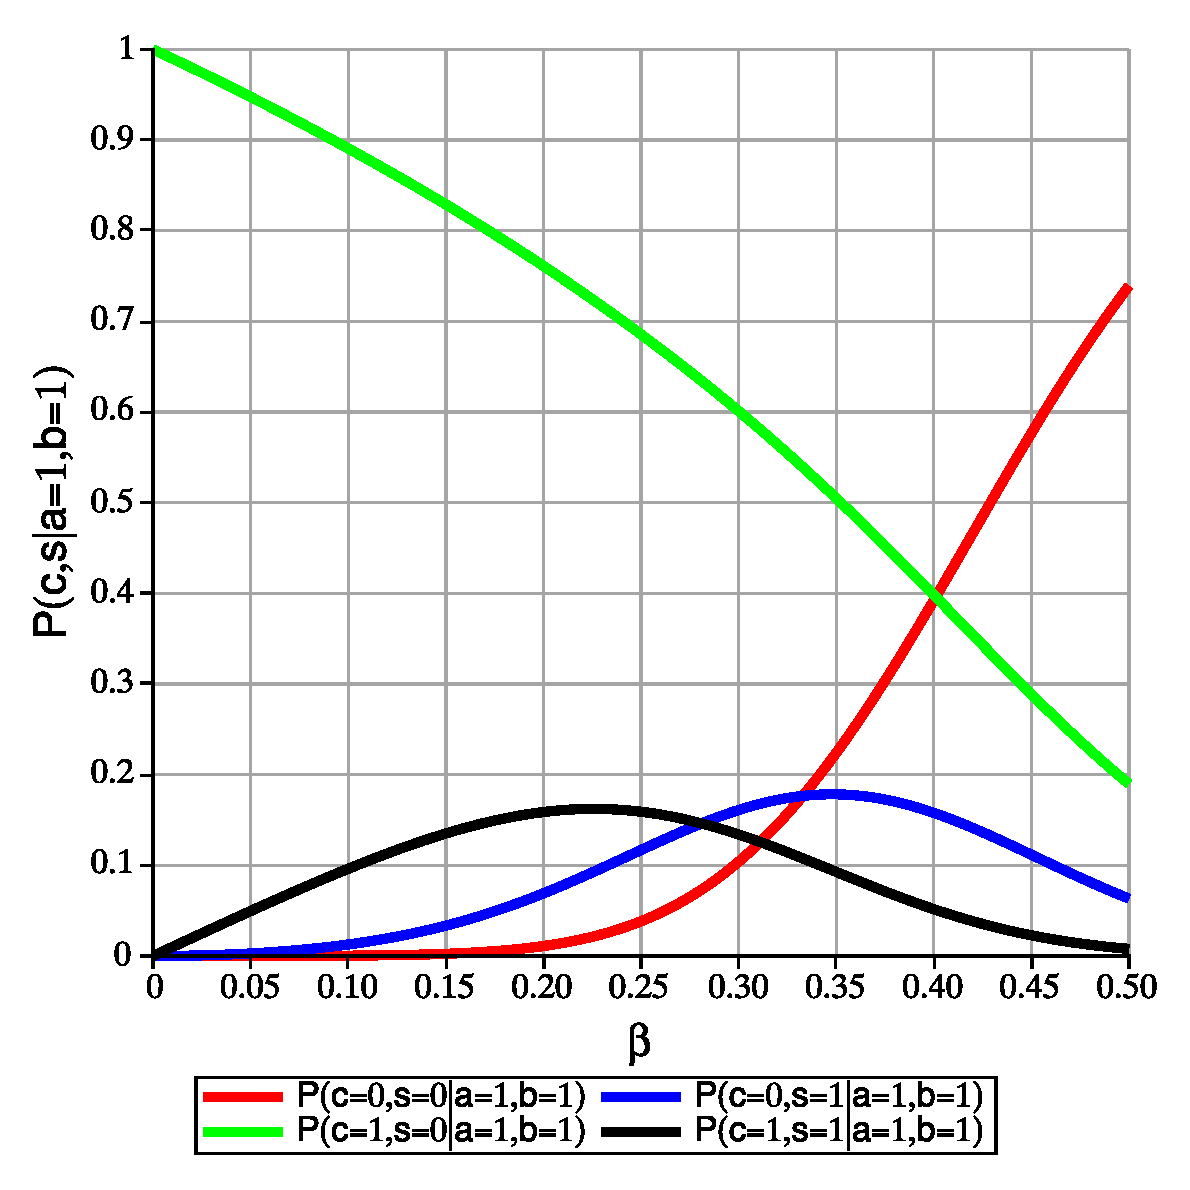
\includegraphics[width=.4\textwidth]{media/noisy_half_adder_16_redundancy_value_dist_11.eps}
        \end{tabular}
    \end{center}
    \caption{Probability distribution for $P(s,c|a,b)$ for the two different cases of $a=1, b=0$ (left)and $a=1, b=1$ (right), respectively. The graphs show the change of the probability distributions as $\beta$ in (\ref{eq:bit_flip_to_0}) varies from $0$ to $\frac{1}{2}$ and $\alpha = 0$; this case is equivalent to assuming there is only leakage of information due to low-voltage. Note the difference to Figure \ref{fig:noise_prob_dist} middle and right. \label{fig:noise_prob_dist_redudancy}}
\end{figure}
